\chapter{Lösungskonzept}\label{loesungskonzept}
Im Fokus des fünften Kapitels steht die Konzeption einer Anwendung im Microservice-Architektur-Stil.

\section{Design Entscheidungen}

Der folgende Abschnitt behandelt die gewählten Technologien für das Lösungskonzept der Microservice-Architektur.

\subsection{Backend}

\subsubsection{Flask}
Für die Entwicklung der Webanwendung in Python wird das Microframework Flask verwendet.
Dieses beinhaltet nur die wesentlichen Funktionalitäten für die Webentwicklung.
Dafür bietet das Framework eine hohe Flexibilität, da die nötigen Bibliotheken vom Entwickler gewählt werden können \cite{flaskdocu} und
es vereinfacht die Erstellung von \acs{api}s durch Blueprints \cite[S.11]{restfulpython}.

Blueprints sind ein Konzept von Flask, welche die Aufteilung von Komponenten einer Webanwendung ermöglichen.
Diese Komponenten können in Form von Routen unterschiedliche Endpunkte mit einer View ausgeben \cite{flaskdocu}.
Dadurch werden die Funktionalitäten der Webanwendung in Endpunkten strukturiert. 
Dies ist ideal für die Ausführung von losen Diensten, die über Endpunkte kommunizieren.

Weiterhin ermöglichen Flask-Abhängigkeiten, wie die Template-Engine Jinja das Rendern von HTML-Templates mit Daten aus der Flask-Anwendung.
Und das Bereitstellen einer standartisierten Schnittstelle \ac{wsgi} über Werkzeugkasten.
Diese ermöglicht die Verwendung der meisten Webserver \cite{flaskdocu}.


\subsubsection{Gunicorn}
Gunicorn ist ein \acs{wsgi}-\acs{http}-Server für Unix, welcher mit den meisten Webframeworks kompatibel ist.
Das Gunicorn-Modell teilt einen Master-Prozess in mehrere Worker-Prozesse auf.
Der Master-Prozess ist lediglich eine Schleife für die bestehenden Worker-Prozesse
und ist bei einem Ausfall für den Neustart zuständig.
Die Worker-Prozesse sind für die Verarbeitung von eingehenden Anfragen zuständig.
Diese teilen sich in folgende Worker-Klassen auf. 
Sync-Workers bearbeiten Anfragen jeweils einzeln und unterstützten keine persistente Verbindung.
Async-Workers basieren auf Greenlets und unterstützten mithilfe von Gevent asynchrone Koroutinen \cite{gunciorndocs}. 

\subsubsection{OpenCV}
OpenCV ist eine Open-Source-Computer-Vision-Bibliothek\footnote{Computer-Vision bezeichnet die Transformation von visuellen Daten in eine abgewandelte Form, die zu Beantwortung einer Fragestellung dienen kann.}, die zur Vearbeitung von Bildern verwendet wird \cite{opencvintro}.
Da ein Video nur eine Serie von Bildern ist, können die Techniken der Bildverarbeitung auch hier genutzt werden \cite{ansari_core_2020}.
Die Bibliothek beinhaltet eine Vielzahl an Algorithmen mit Bezug zu Computer Vision oder Machine Learning.
Diese untersützten auch die Verwendung von \acp{gpu} die auf den Programmierschnittstellen \ac{cuda} oder \ac{opencl} basieren \cite{opencvpython}.
Die Anwendung wird mit der Python-Version der Bibliothek entwickelt, um die Implementierung in die Python-Webanwendung zu vereinfachen.



\subsection{Frontend}

\subsubsection{\ac{html} und JavaScript}
Die Umsetzung der Benutzerobfläche erfolgt mit der Auszeichnungssprache \acs{html}5 in Kombination
mit der Skriptsprache JavaScript, um Interaktion mit dem Anwender zu ermöglichen.
Für die erleichterte Gestaltung der Website wird das Frontend-\acs{css}-Framework Bootstrap in der Version 5.0 genutzt.

\subsection{Kommunikation}

\subsubsection{Socket.IO}
Die bidirektionale und ereignisbasierte Echtzeitkommunikation zwischen den Diensten wird mithilfe der Bibliothek Socket.IO realisiert.
Die Bibliothek unterstützt mehrere Programmiersprachen für Server- und Client-Implementierungen, welche von der Community gewartet werden.
Eine Kommunikation zwischen Server und Client erfolgt über WebSockets. 
Wenn dies nicht möglich ist, wird auf die ressourcenintensivere \cite{httpwebsocket} Alternative \acs{http}-long-polling zurückgegriffen \cite{socketio}.
Für die Kommunikation der Webanwendung wird die Server Implementierung von Python-Socketio genutzt \cite{python-socketio}.
Die Implementierung der Anwendungslogik erfolgt über die Plattformunabhängige JavaScript-Bibliothek Socket.IO.


\subsubsection{\ac{rest}}
\acs{rest} ist eine auf Ressourcen basierende Architektur für verteilte Systeme.
Diese Ressourcen werden über eine einheitliche Schnittstelle basierend auf 
\acs{http} Methoden zugänglich gemacht.
Dabei ist jede Ressource über eine URL erreichbar.
REST erlaubt dabei Ressourcen in verschiedene Datentypen zu repräsentieren, wie Text, XML, JSON etc.
Die CRUD-Funktionen (create, read, update und delete) werden über die HTTP-Methoden GET, POST, PUT und DELETE realisiert \cite{fundamentalsRestfulAPI}.
\subsection{Datenbank}

\subsubsection{MongoDB}

MongoDB ist eine dokumentenorientierte Datenbank, bei der Daten nicht in einer Tabelle, 
sondern in Dokumenten gespeichert werden.
Sie zählt damit zu den NoSQL-Datenbanken.
Die Dokumentenorientierung ermöglicht die Darstellung von komplexen hierarchischen Beziehungen mit einem einzigen Eintrag.
Dokumente sind nach einer Key-Value-Struktur aufgebaut und besitzen kein vorgeschriebenes Schema zur Erstellung von Einträgen \cite{mongodbdefinitive}.

\subsection{Versionsverwaltungssystem}
\subsubsection{GitHub}
Das verwendete Versionsverwaltungssystem für die Entwicklung der Microservices ist GitHub.
Dieses basiert auf git und fokusiert sich auf Open-Source-Software und bietet gleichzeitig Enterprise-Support für Unternehmen \cite{githubpricing}.
Die Krones AG hat die Möglichkeit GitHub für zukünftige Entwicklungsprozesse von Microservices zu verwenden.

\subsubsection{DockerHub}
Wie in Abschnitt \ref{Docker} beschrieben ist die Standard-Registry für Docker-Images DockerHub.
Deshalb werden für die Bereistellung der Docker-Images die kostenfreien und öffentlichen Repositories verwendet.
Die Entwicklung der Dienste erfolgt in getrennten Repositories.

\section{Entwicklung}
In dem folgenden Abschnitt werden die Entwicklungsschritte der Microservice-Anwen\-dungen und der Ressourcenobjekte für das Bereitstellen mit Helm näher erläutert.


\subsection{Microservice-Entwicklung}
Die Abbildung \ref{fig:DevWorkflowDocker} zeigt den Arbeitsablauf der Service-Entwicklung auf.
Zuerst wird die Funktionalität des Dienstes realisiert und dann mithilfe eines Dockerfiles ein Docker-Image erstellt.
Dafür wird ein Base-Image entweder aus einem Docker-Registry, wie DockerHub, oder aus dem lokalen Registry benötigt.
Um den Container zu starten, kann ein Docker-Befehl auf dem Hostssystem ausgeführt werden.
Die Nutzung von Tools wie Docker-Compose erlauben das Starten mehrerer Container mithilfe von Konfigurationsdateien in Form von YAML-Dateien.
Nach dem Ausführen der Container können diese getestet werden.
Abschließend kann der Entwicklungsablauf fortgeführt werden oder ein Release für das Versionsverwaltungssystem und das Container-Repository erstellt werden.


\begin{figure}[!htb]
    \centering
    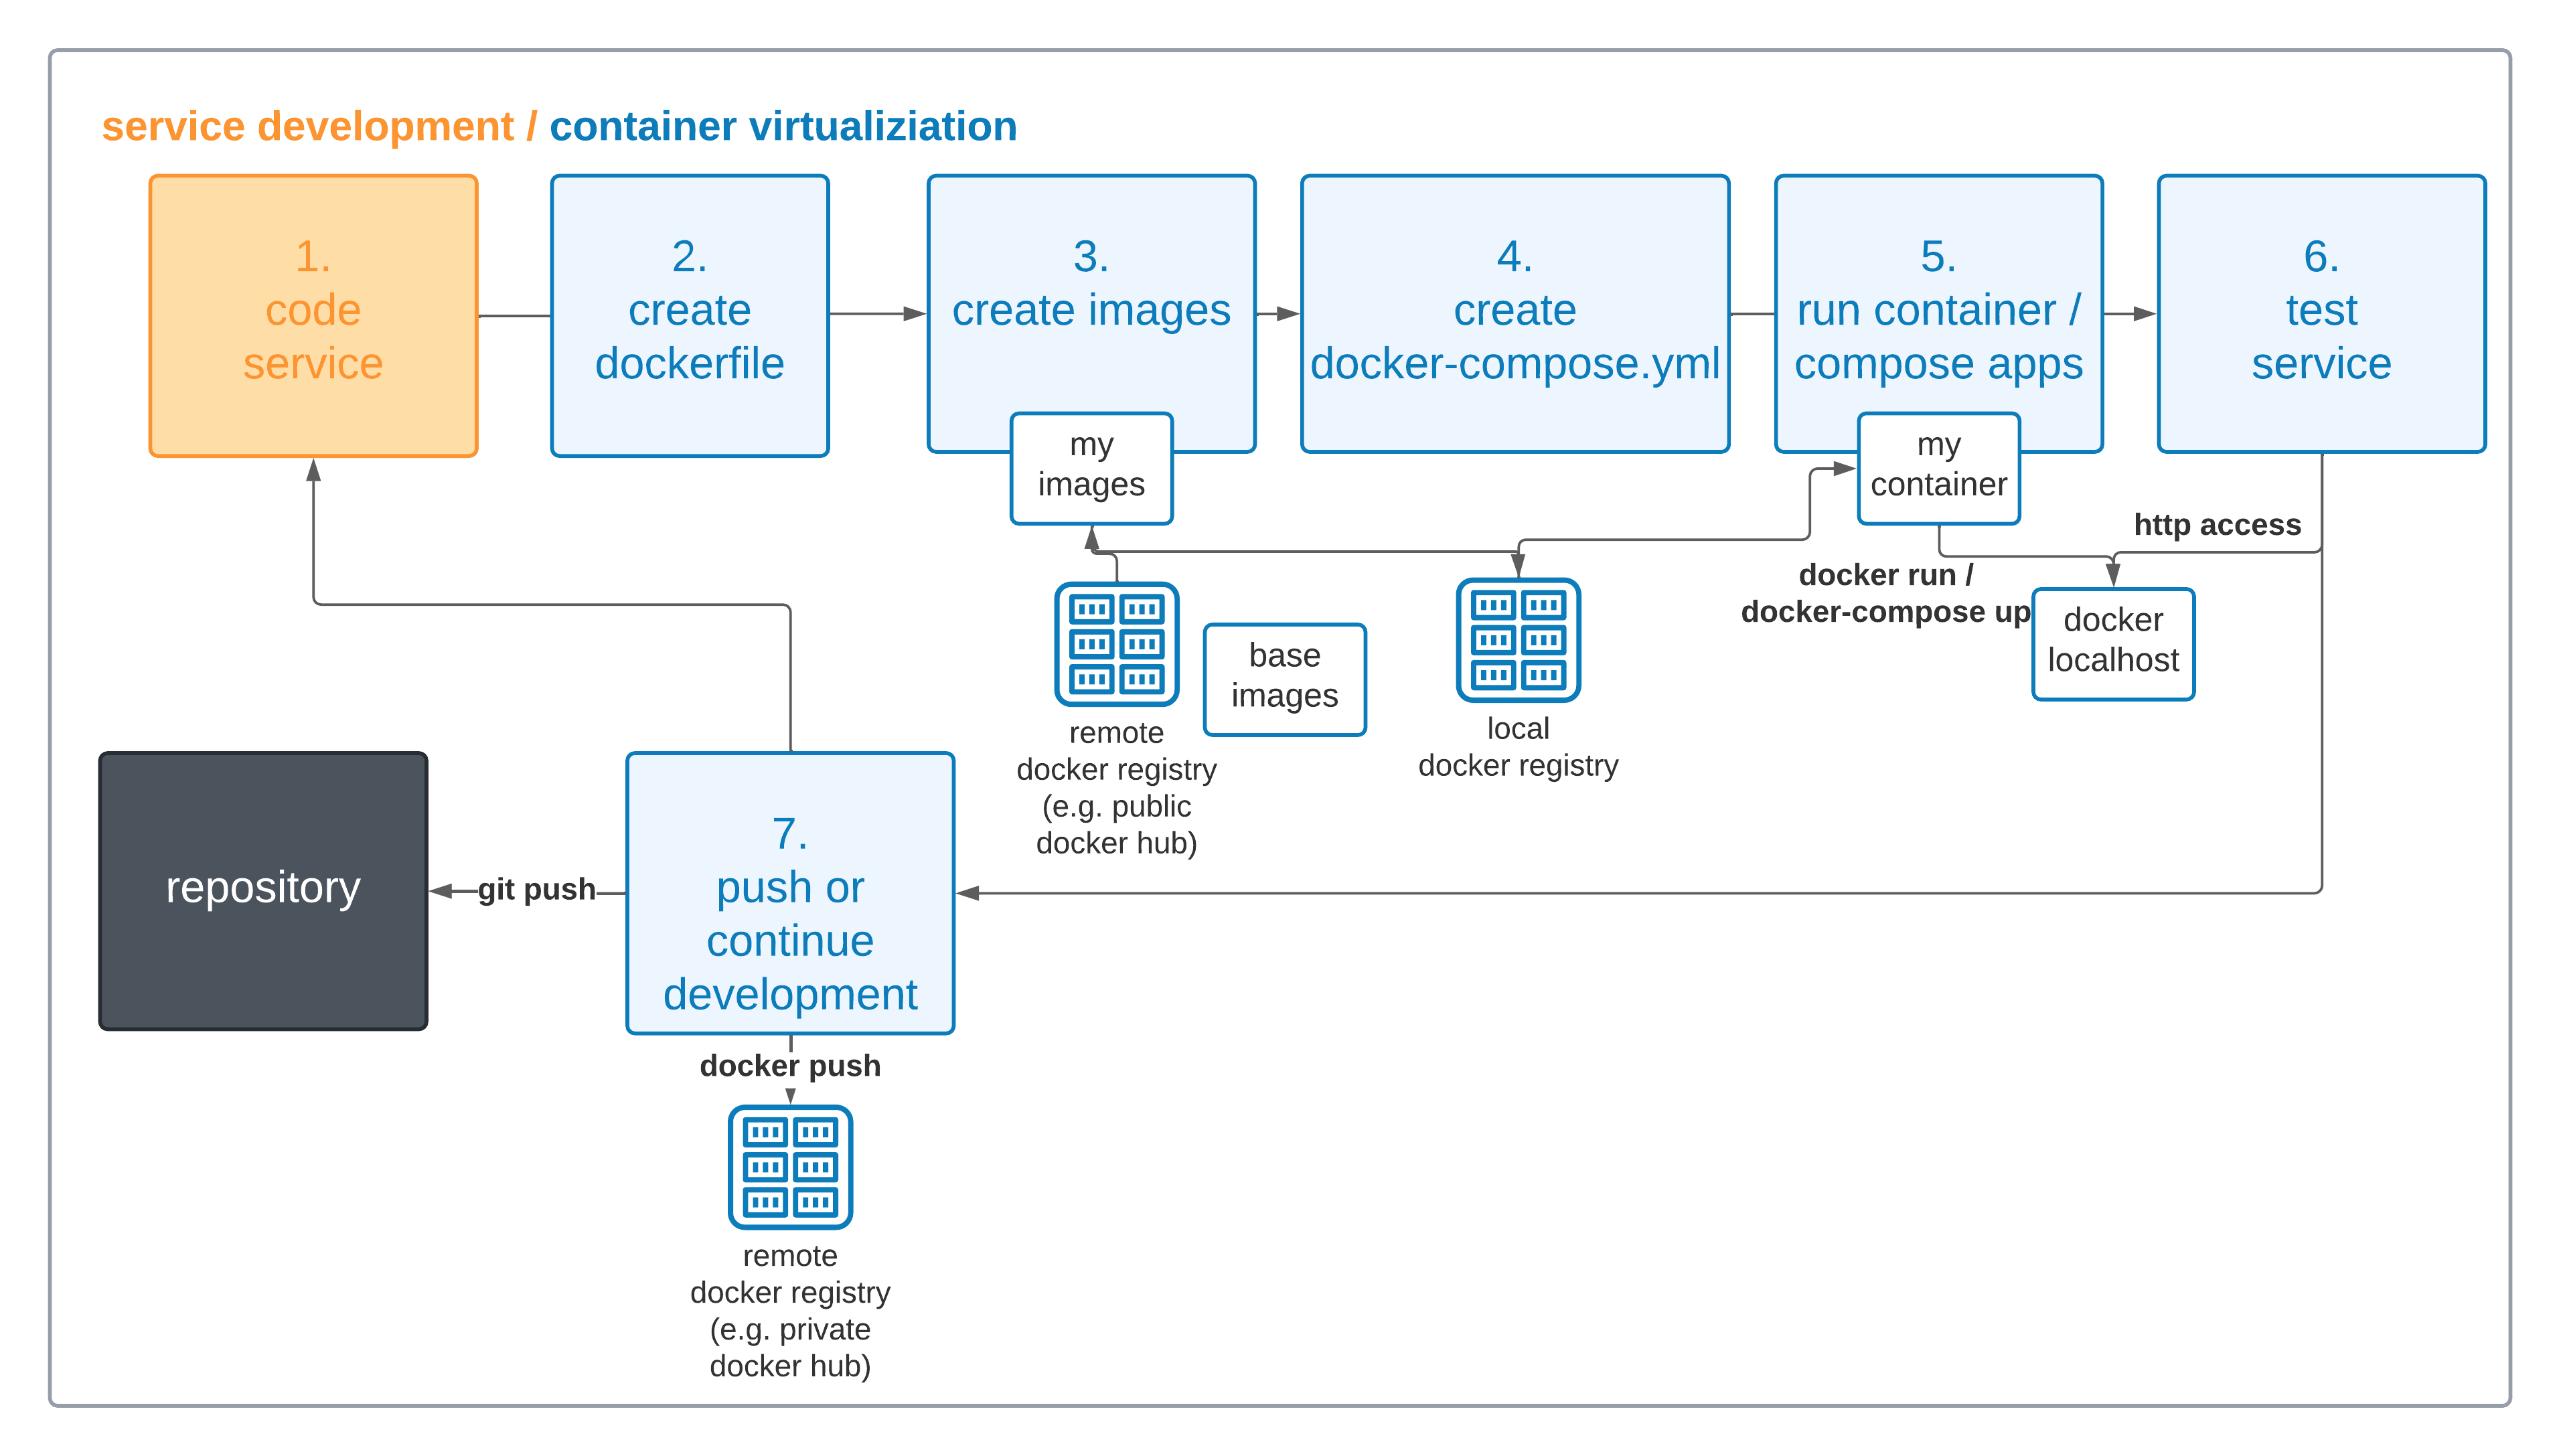
\includegraphics[width=1.0\columnwidth]{images/DevWorkflowDocker.png}
    \caption{Microservice-Entwicklung in Anlehnung an \cite{dockerappsworkflow}}
    \label{fig:DevWorkflowDocker}
\end{figure}


\subsection{Helm-Chart-Entwicklung}

Die Abbildung \ref{fig:DevWorkflowKubernetes} beschreibt den Vorgang bei der Entwicklung von Helm-Charts für Kubernetes.
Als Erstes wird ein Helm-Chart entwickelt.
Der Kommandozeilenbefehl \textit{helm lint} überprüft den vorgegebenen Pfad zum Chart und führt eine Serie von Tests zur Validierung durch.
Danach kann dieser auf einem Kubernetes-Cluster installiert werden, 
wenn die Kubernetes-Ressourcenobjekte einen Docker-Container benötigen,
wird das spezifizierte Image aus dem öffentlichen DockerHub-Registry heruntergeladen.
Der Service kann jetzt mit dem Kommandozeilentool Kubectl getestet werden.
Zuletzt wird die Entwicklung am Helm-Chart fortgeführt oder das Egebnis Artefakt ins Versionsverwaltungssystem hochgeladen.


\begin{figure}[!htb]
    \centering
    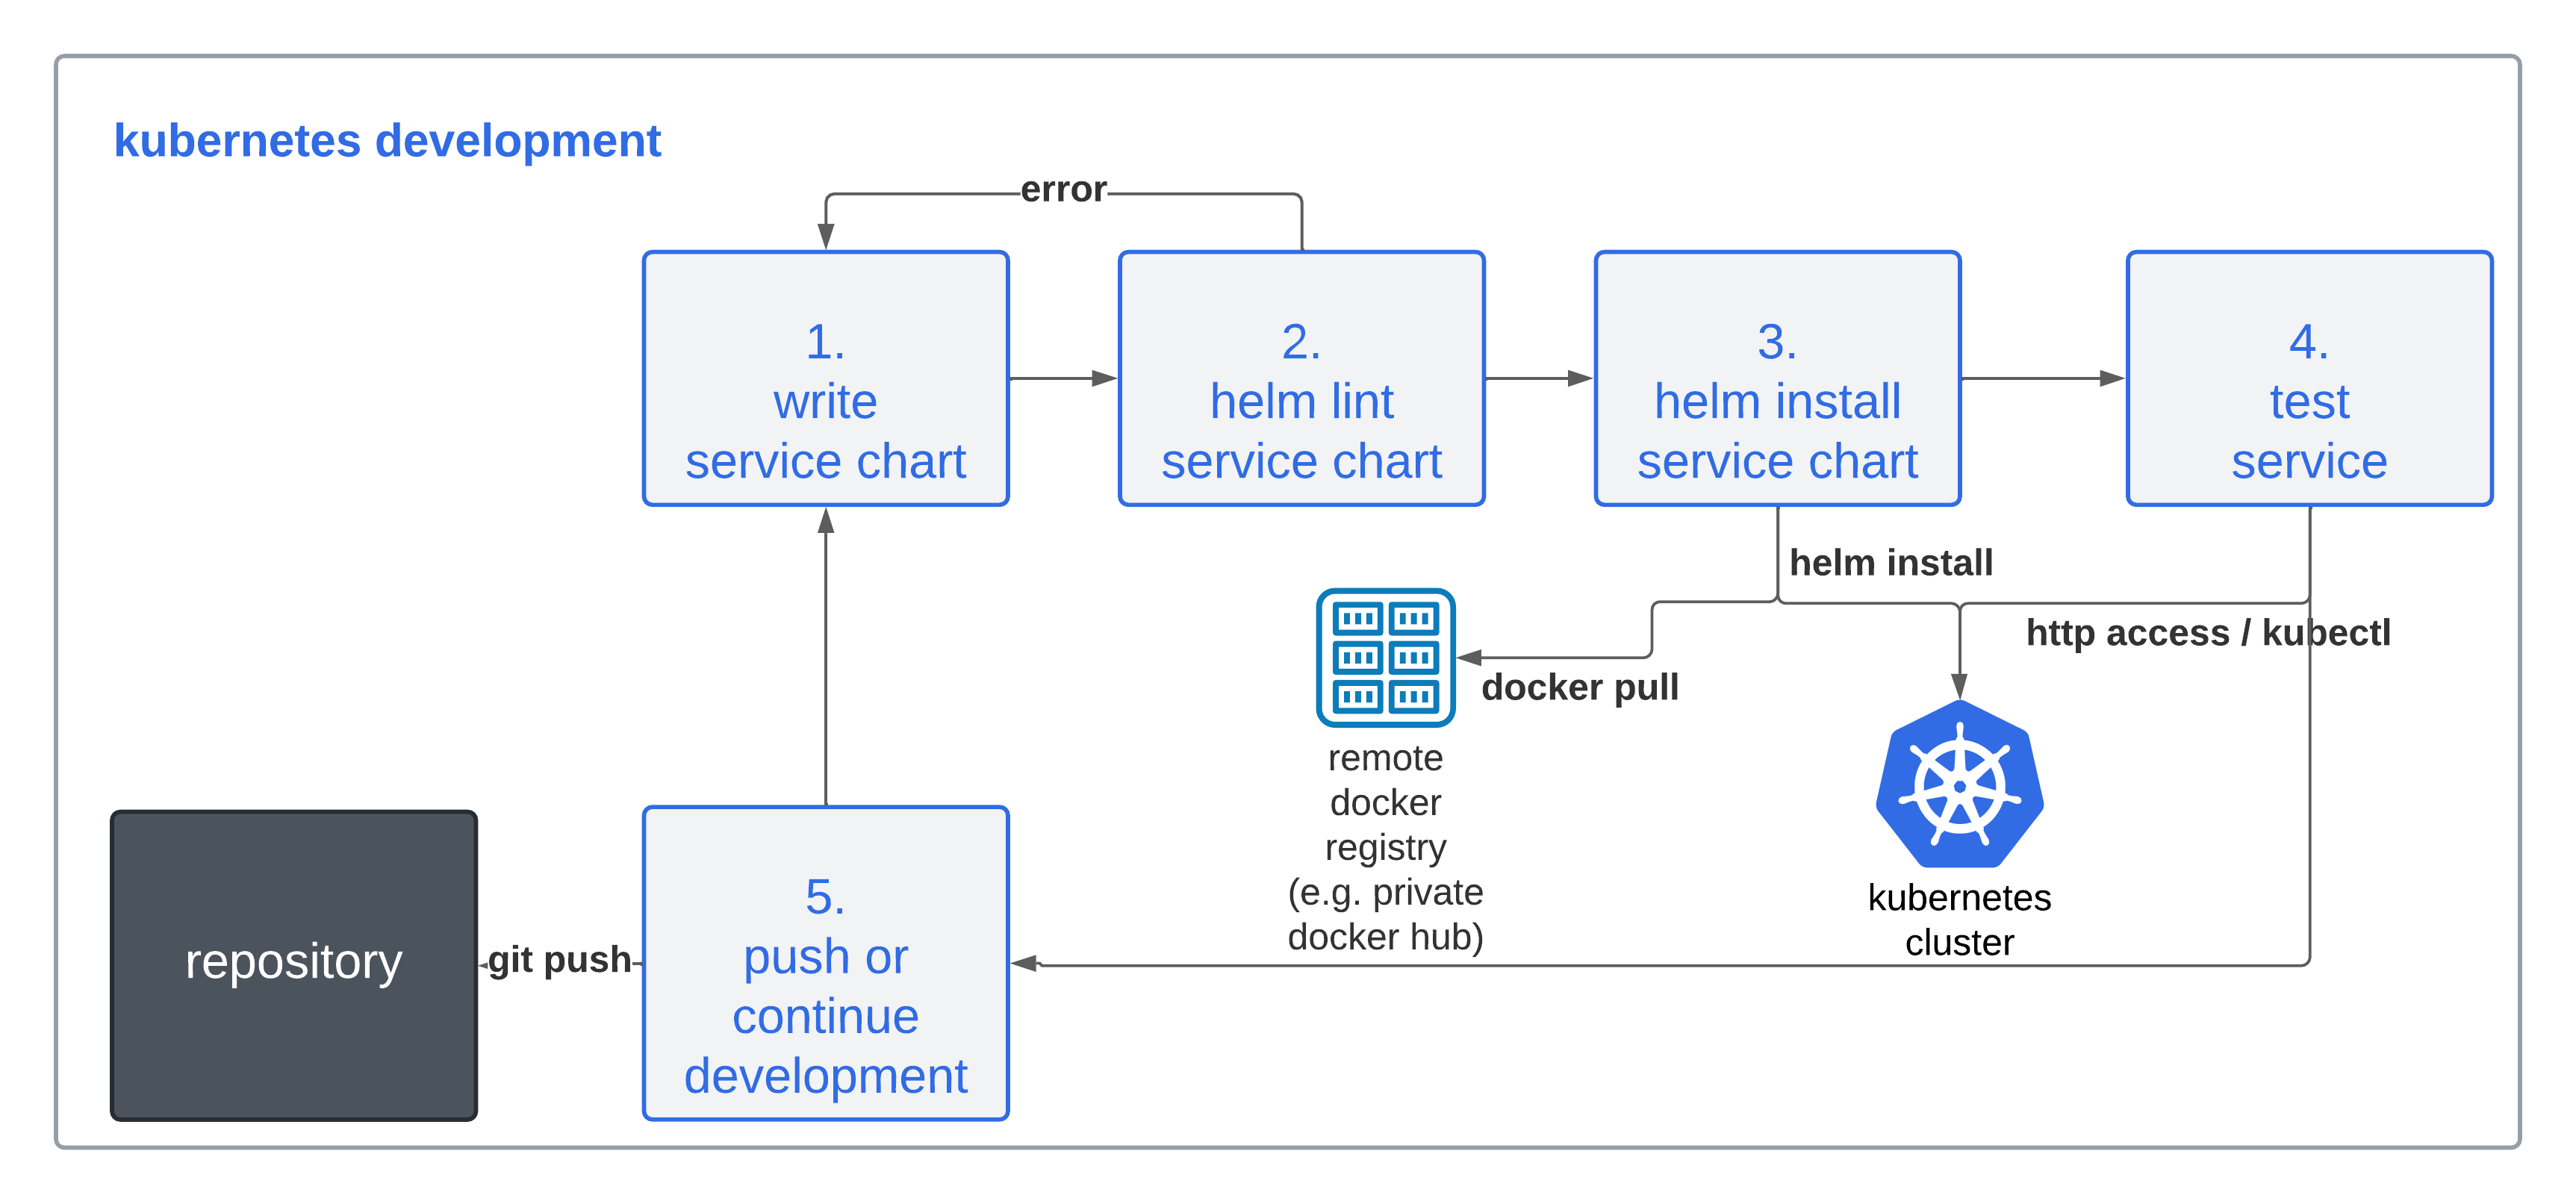
\includegraphics[width=1.0\columnwidth]{images/DevWorkflowKubernetes.png}
    \caption{Kubernetes-Entwicklung in Anlehnung an \cite{dockerappsworkflow}}
    \label{fig:DevWorkflowKubernetes}
\end{figure}


\newpage
\section{Architektur}
Dieser Abschnitt befasst sich mit der Architektur der zu entwickelnden Anwendung.
Die Aufgaben der einzelnen Dienste der Microservice-Architektur wurden konzipiert und dargestellt.
Danach folgt der Vorgang der Installation der losen Dienste mit Helm auf dem Kubernetes-Cluster.

\subsection{Microservices}

Die Abbildung \ref{fig:UML-Microservices} zeigt die einzelnen Softwarekomponenten der Webanwendung, welche als Docker-Container laufen.
Das Frontend dient als visuelles Gateway für die anderen Dienste.
Dieses bietet vier Endpunkte, die für Nutzer über einen Webbrowser erreichbar sind.
Der Home-Endpunkt ermöglicht den Login oder Logout eines Nutzers über die REST-API des Authentication-Dienstes.
Register erlaubt die Registrierung eines Nutzers in der Datenbank.
Train und Facelogin senden Bilder an den Facerecognition-Dienst, dies geschieht mit dem Kommunikationsprotokoll SocketIO.
Damit wird das Modell zur Gesichtserkennung trainiert und ermöglicht die spätere Zwei-Faktor-Authentifizierung mittels Login per Gesichtserkennung.


\begin{figure}[!htb]
    \centering
    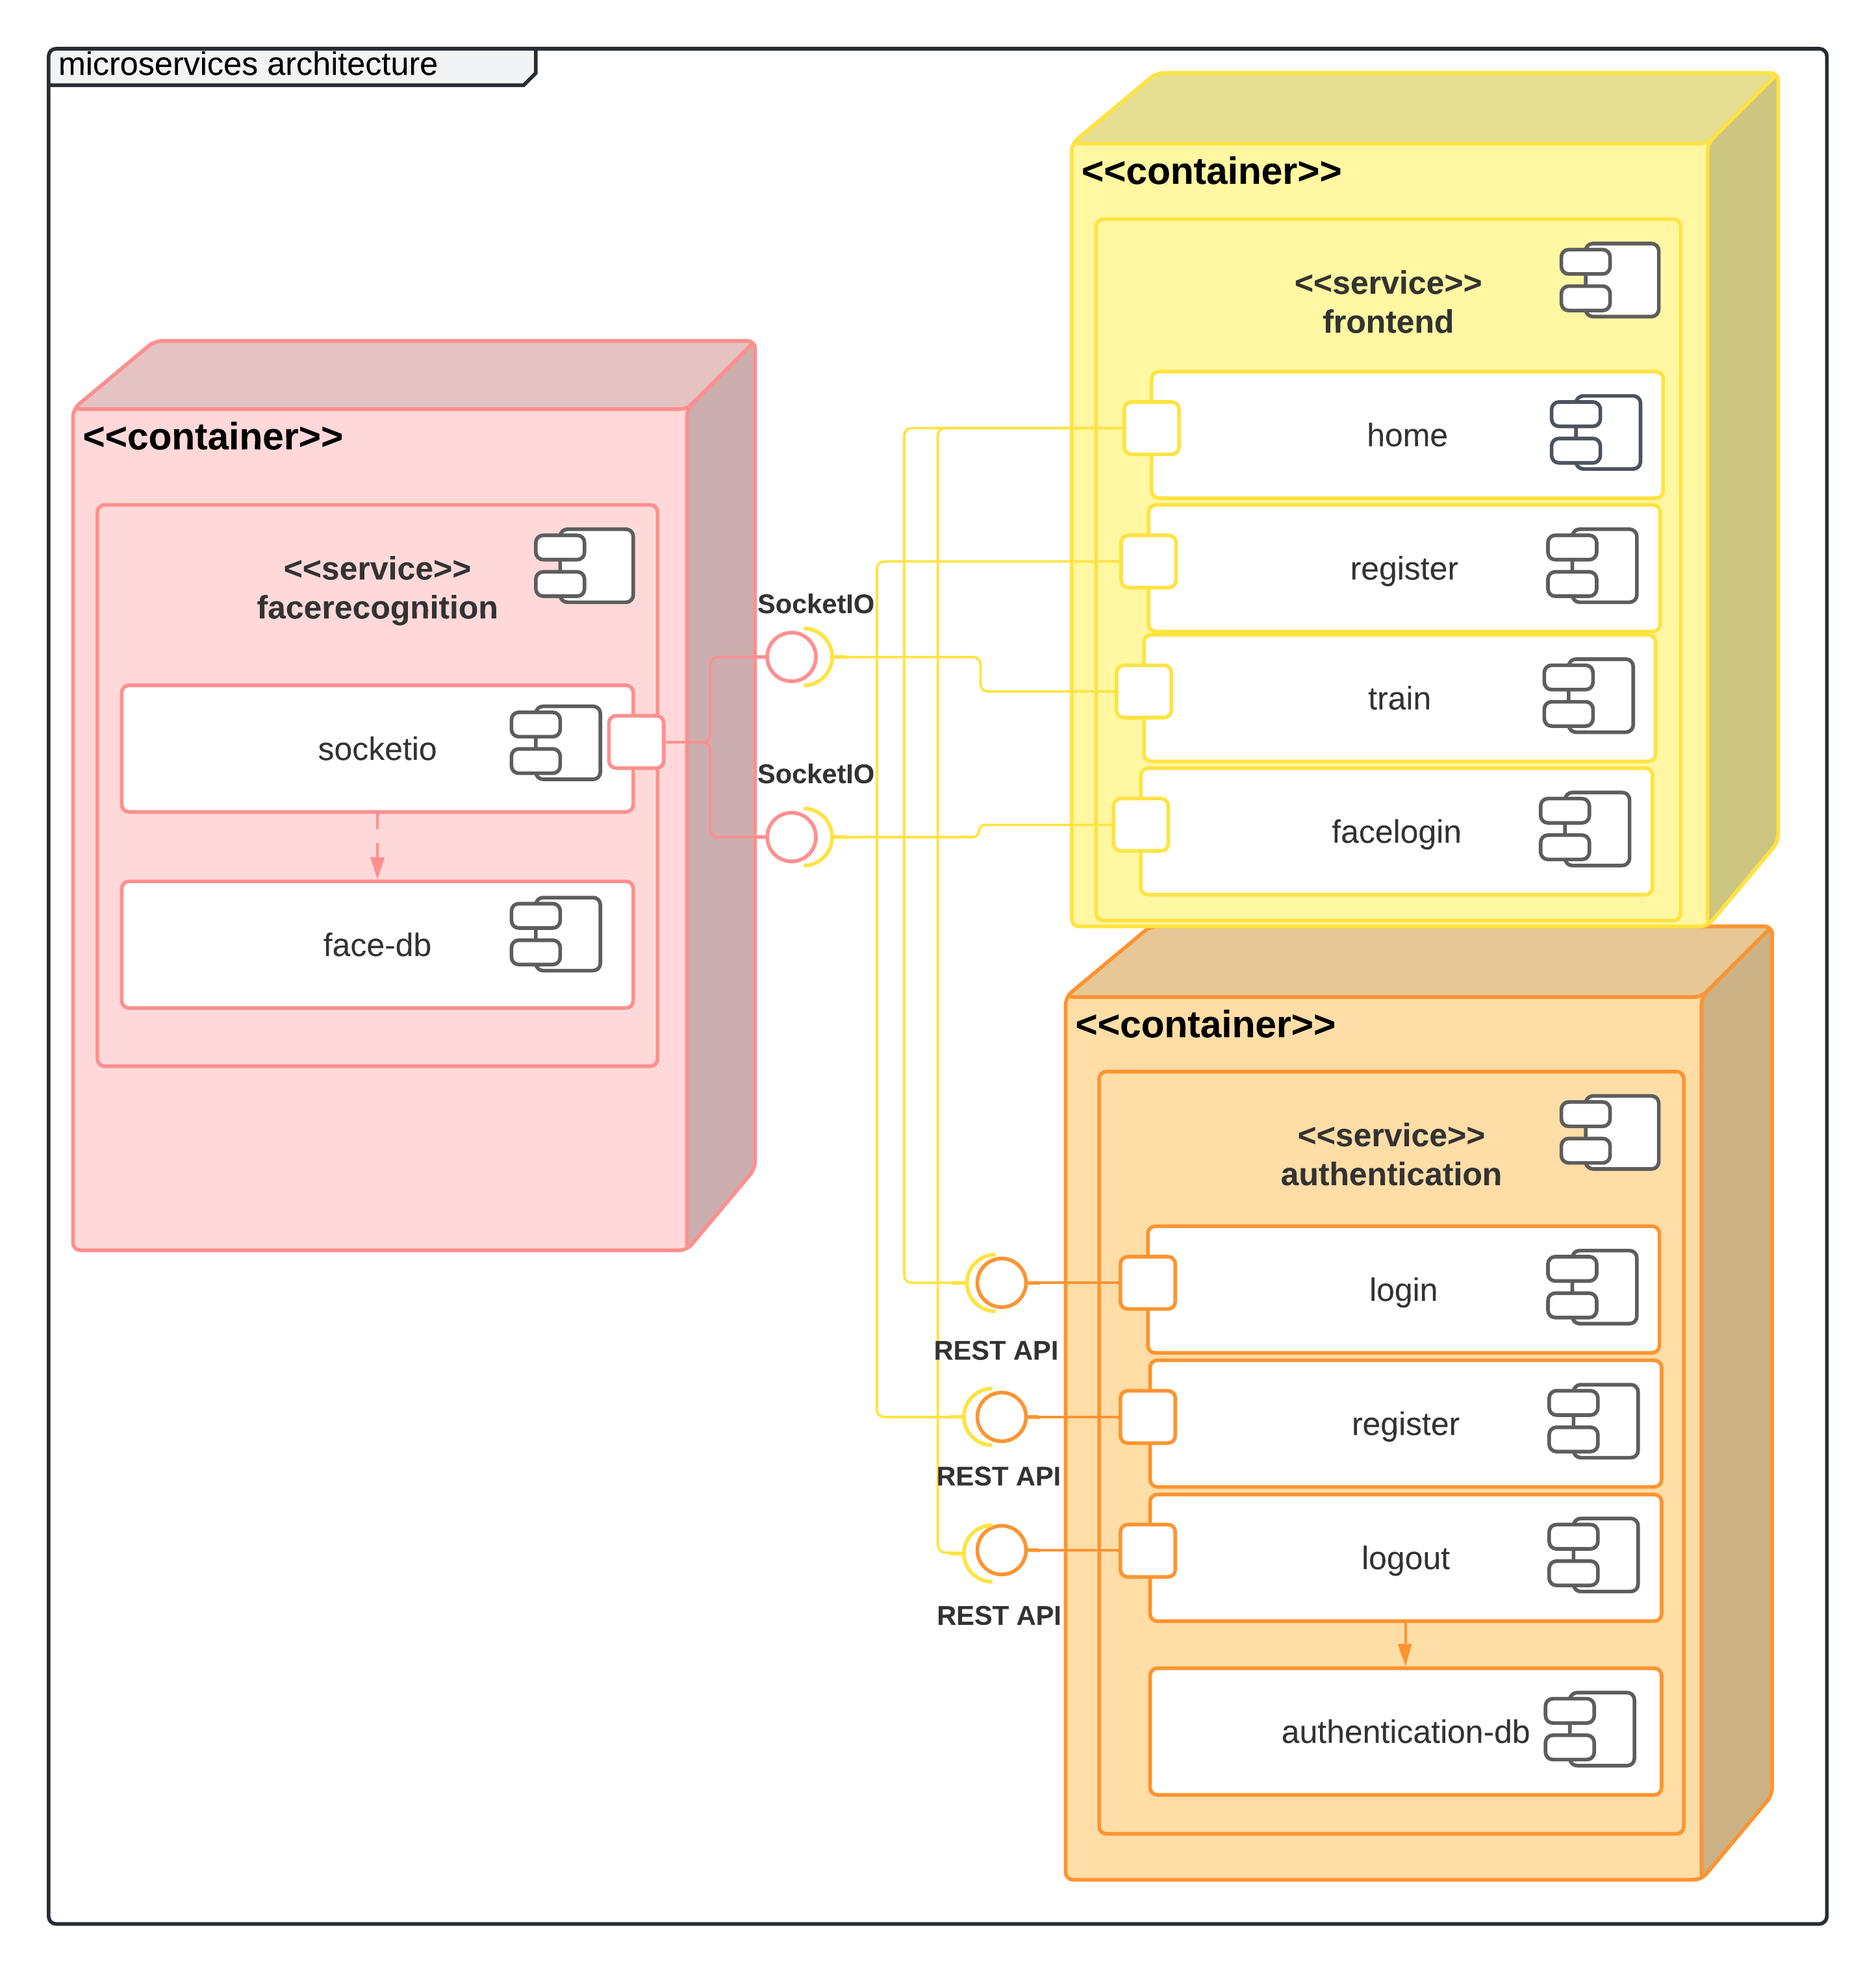
\includegraphics[width=1.0\columnwidth]{images/UML-Microservices-Diagramm.png}
    \caption{Lokale Microservice Entwicklung}
    \label{fig:UML-Microservices}
\end{figure}




\subsection{Helm-Installation}

Die einzelnen Dienste der Webanwendung werden mithilfe von einem Helm-Chart gleichzeitig auf ein Kubernetes-Cluster installiert.
Dabei hat jeder Dienst ein eigenes Verzeichnis mit den notwendigen Kubernetes-Ressourcenobjekten.
Der Zugang erfolgt über eine Kubeconfig die den Zugang zum Kubernetes-Cluster ermöglicht.
Bei erfolgreichem Zugang kann mit einem Befehl im Verzeichnis die Microservices installiert werden.
Das Kubernetes-Cluster bezieht dann die benötigten Docker-Images aus den angegebenen Docker-Repositories.
Die erfolgreiche Bereistellung der Container auf dem Cluster ist dann unabhängig von der Helm-Installation, wenn die Images nicht von den angegebenen Repositories bezogen werden können. 
Die Bereistellung und Auslieferung der Kubernetes-Ressourcenobjekte ist trotzdem erfolgreich und gibt auf dem Kubernetes-Cluster lediglich Fehlermeldungen, bei der versuchten Ausführung der Container in einem Pod an.

\begin{figure}[!htb]
    \centering
    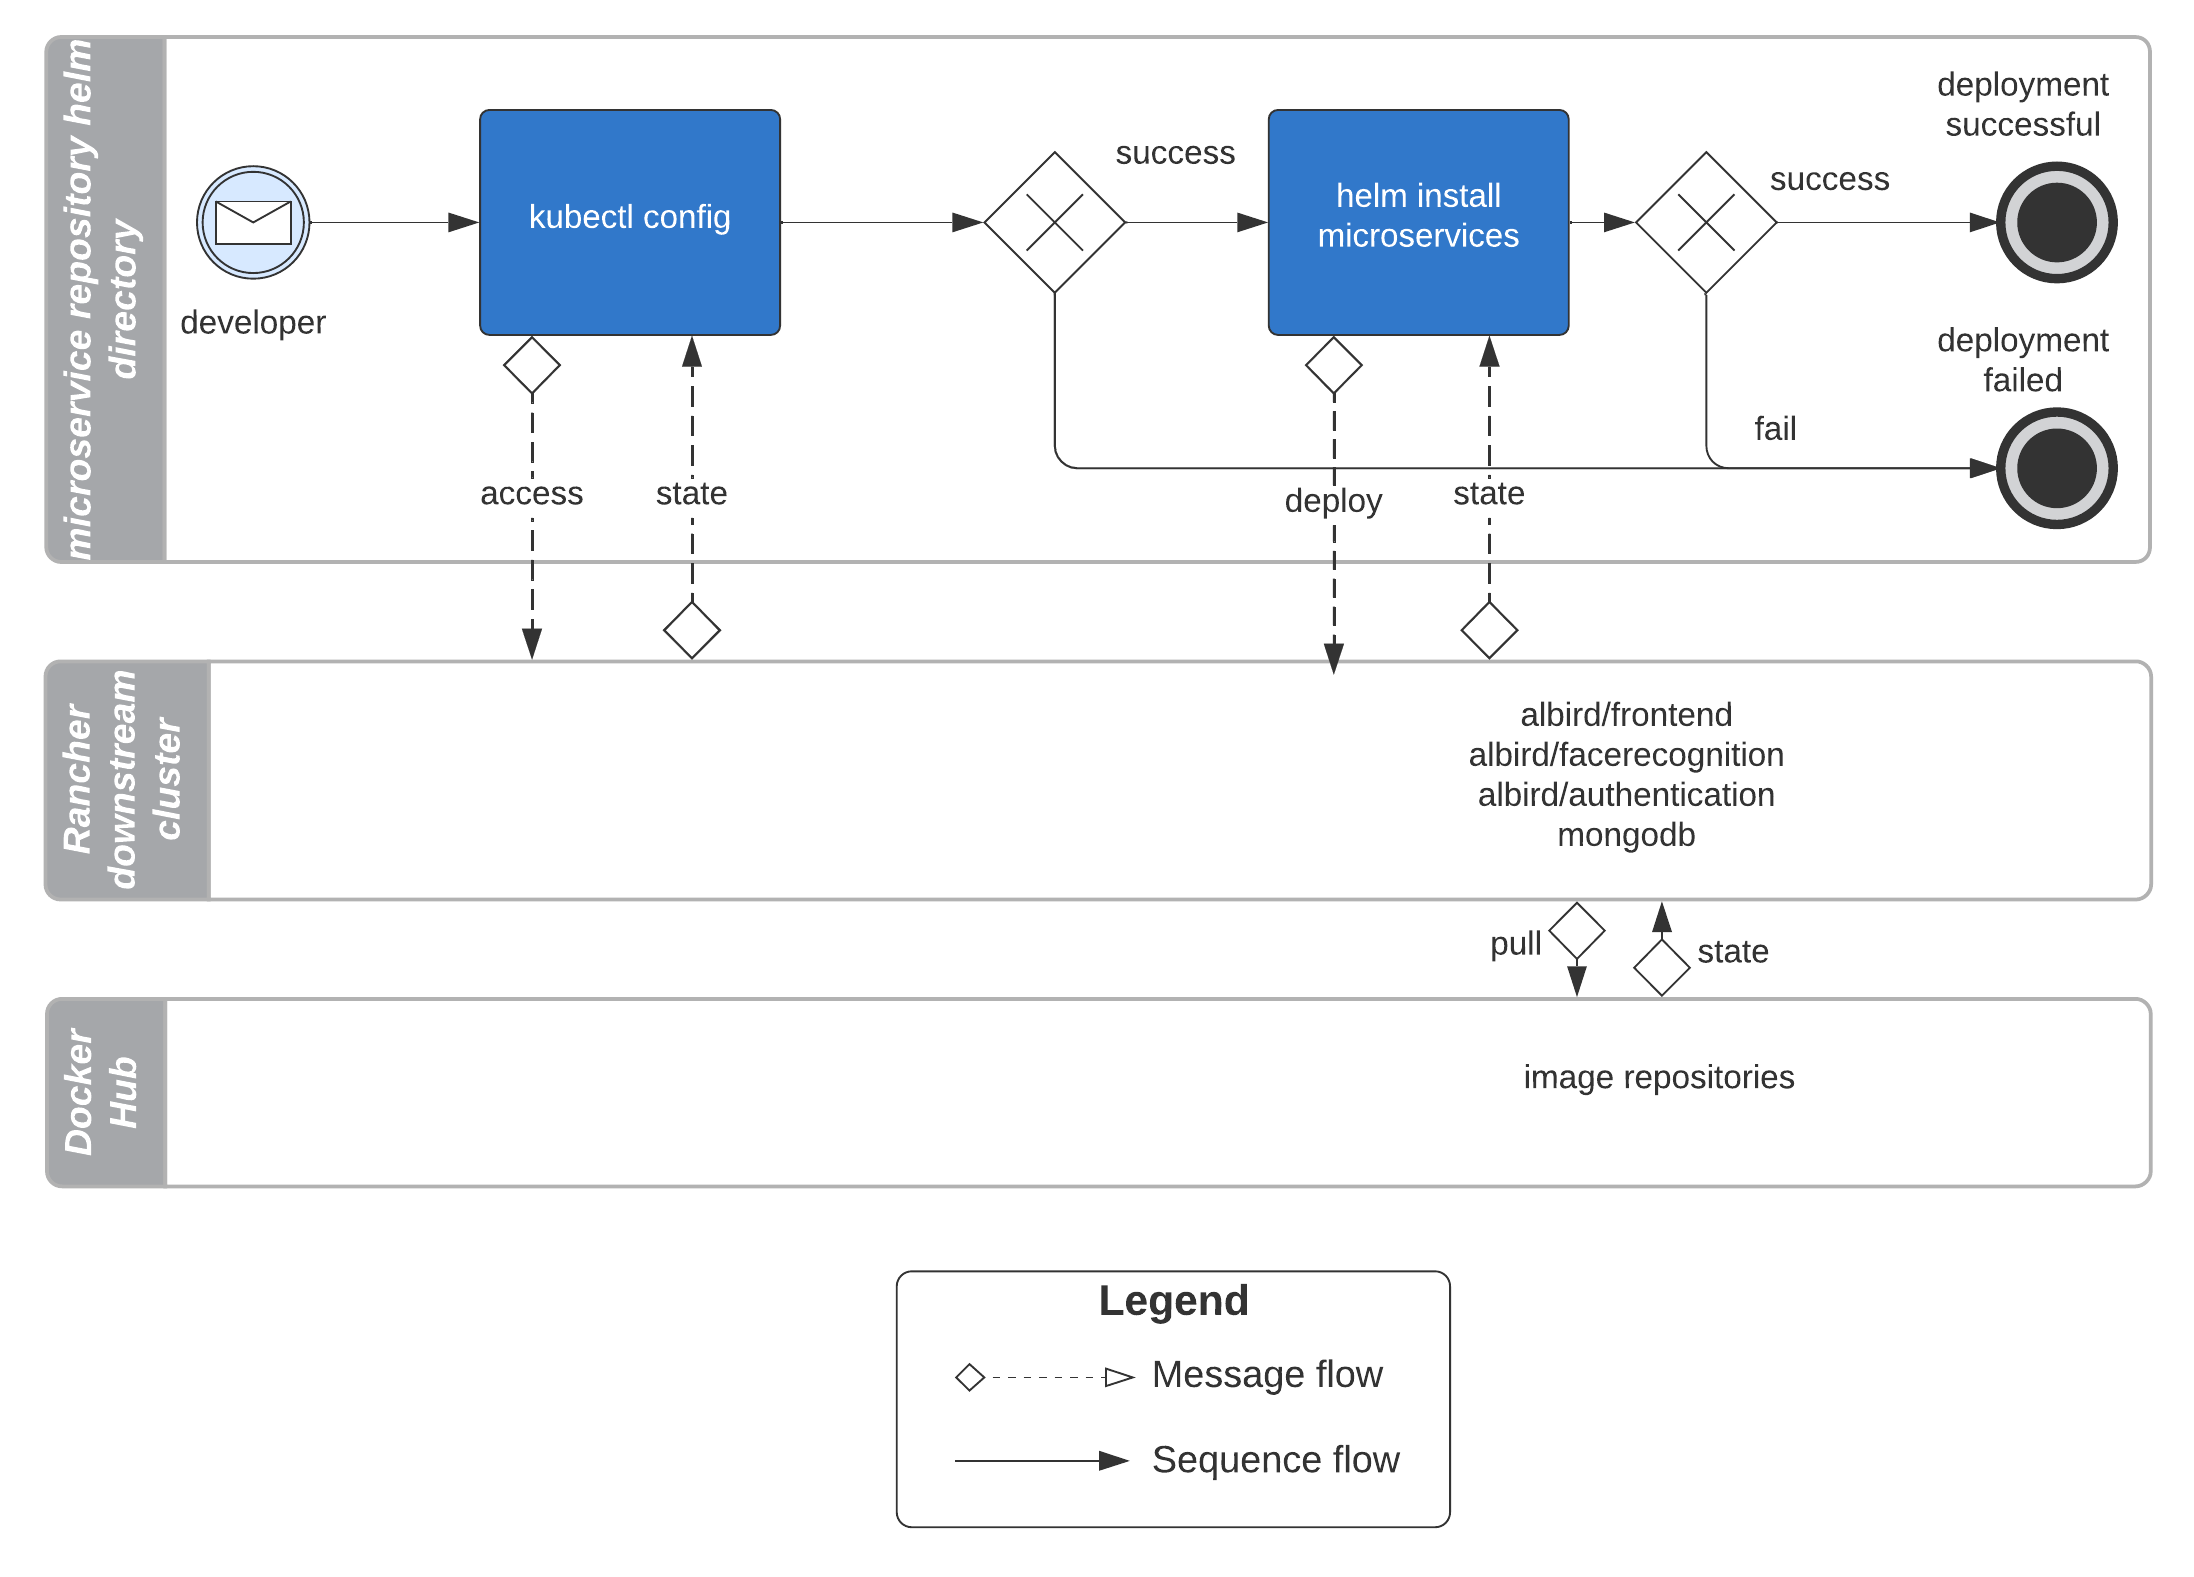
\includegraphics[width=1.0\columnwidth]{images/BPMNHelm.png}
    \caption{BPNM Modell - Helm--Installation der Microservices}
    \label{fig:HelmInstallation}
\end{figure}





